\begin{figure}[t]
	\centering
    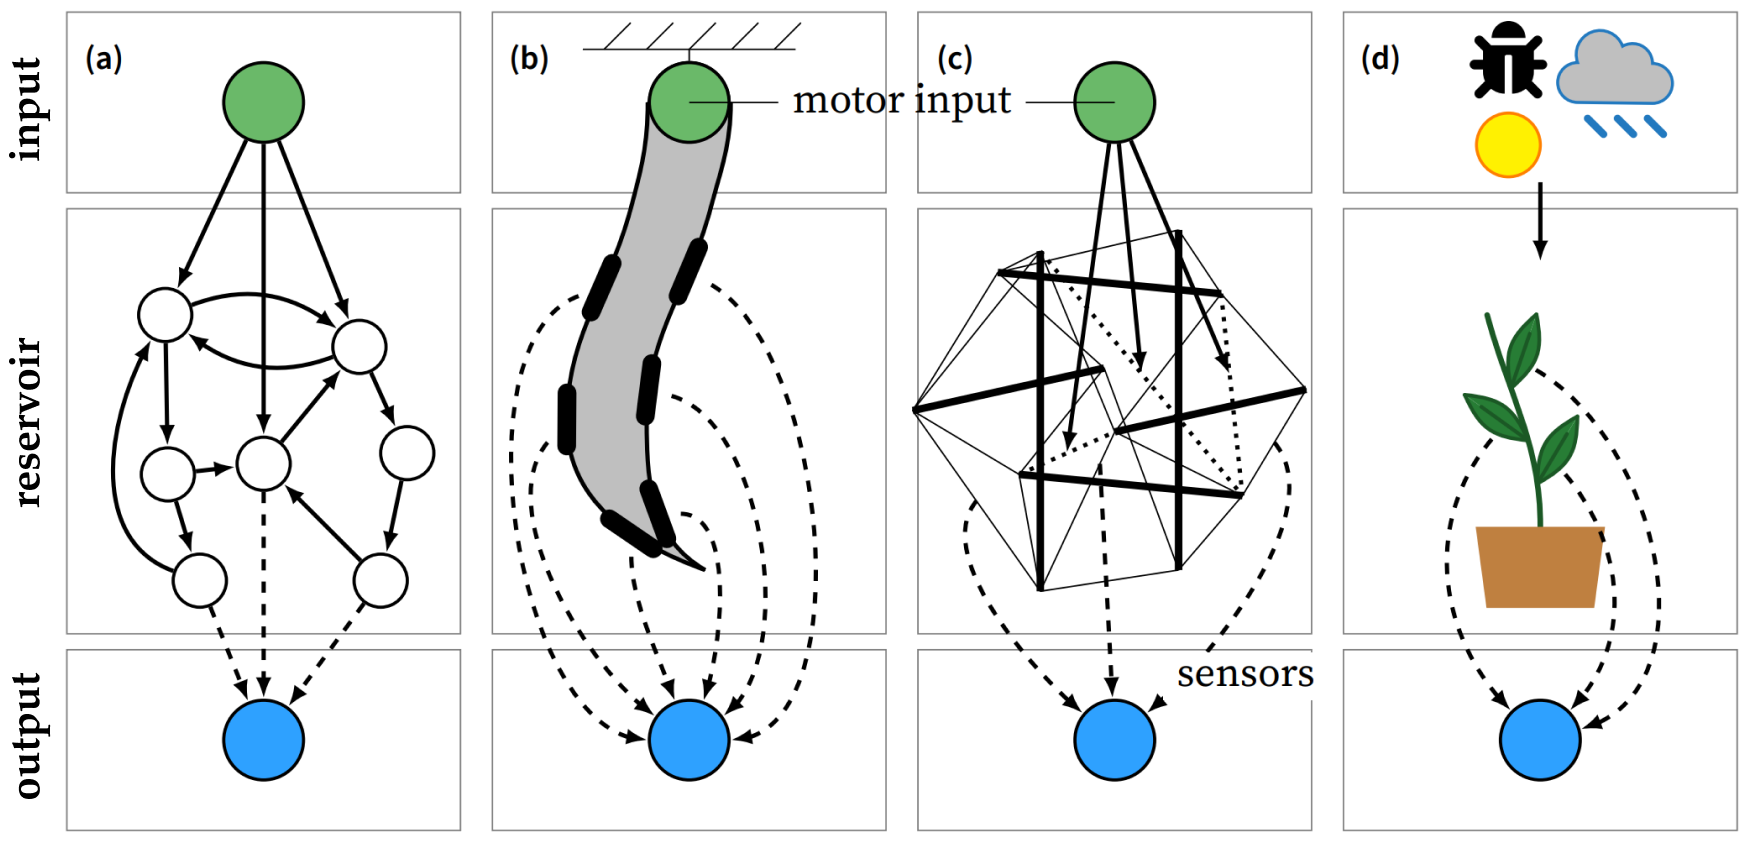
\includegraphics[width=0.9\textwidth]{img/prc-illustration.png}
    % \vspace{0.5cm}
    % \includegraphics[width=0.5\textwidth]{example-image}
	\caption[Illustration of different reservoir computing implementations, both theoretical and physical versions.]
	        {Illustration of different reservoir computing implementations, both theoretical and physical versions. 
	        Each of the subfigures depicts a different type of implementation: 
	            (a) RNN-based version; 
	            (b) soft body built of silicone \citep{nakajima_information_2015}; 
	            (c) compliant robot made of a tensegrity structure \citep{caluwaerts_locomotion_2013}; 
	            and (d) plant as reservoir.
    	 	Figure and caption reused from \citet{pieters_reservoir_2022} with permission from the author.}
	\label{fig:prc_examples}
\end{figure}